% This LaTeX document needs to be compiled with XeLaTeX.
\documentclass[10pt]{article}
\usepackage[utf8]{inputenc}
\usepackage{hyperref}
\hypersetup{colorlinks=true, linkcolor=blue, filecolor=magenta, urlcolor=cyan,}
\urlstyle{same}
\usepackage{amsmath}
\usepackage{amsfonts}
\usepackage{amssymb}
\usepackage[version=4]{mhchem}
\usepackage{stmaryrd}
\usepackage{graphicx}
\usepackage[export]{adjustbox}
\graphicspath{ {./images/} }
\usepackage[fallback]{xeCJK}
\usepackage{polyglossia}
\usepackage{fontspec}
\usepackage{newunicodechar}
\setCJKmainfont{Noto Serif CJK SC}

\setmainlanguage{german}
\setmainfont{CMU Serif}

\author{Articles\\
Title Summary\\
- Article 1 X\\
Article 1 Summary\\
- Article $2 \boldsymbol{X}$\\
- Article $3 \boldsymbol{X}$\\
- Article $4 \underline{X}$}
\date{}


\newunicodechar{ı}{\ifmmode\imath\else{$\imath$}\fi}

\begin{document}
\maketitle
\section*{WBE: Ul-BIBLIOTHEK}
\section*{TEIL 3: EINSATZ}
\section*{ÜBERSICHT}
\begin{itemize}
  \item Zustand von Komponenten
  \item Komponenten-Design
  \item Optimierungsansätze
\end{itemize}

\section*{ÜBERSICHT}
\begin{itemize}
  \item Zustand von Komponenten
  \item Komponenten-Design
  \item Optimierungsansätze
\end{itemize}

\section*{ZUSTAND}
\begin{itemize}
  \item Komponenten sollen auch einen Zustand haben können
  \item In React möglich, zum Beispiel mit als Klassen implementierten Komponenten
  \item Neuere Variante: Hooks, in diesem Fall: State-Hook
\end{itemize}

\section*{STATE-HOOK IN REACT}
const [stateVar, setStateVar] = useState(initialValue)

\begin{itemize}
  \item useState liefert Zustand und Update-Funktion
  \item Initialwert wird als Argument übergeben
  \item Zustandsänderung führt zum erneuten Rendern der Komponente
\end{itemize}

\section*{STATE-HOOK IN REACT}
\begin{verbatim}
const Counter = () => {
    const [state, setState] = useState(1)
    const handler = () => setState(c => c + 1)
    return (
        ["h1", {onclick:handler, style:{userSelect:"none",cursor:"pointer"}},
            "Count: " + state]
    )
}
const element = [Counter]
\end{verbatim}

\section*{STATE-HOOK: UMSETZUNG}
\begin{itemize}
  \item Aktuelles Element erhält ein Attribut hooks (Array)
  \item Beim Aufruf der Komponente wird useState aufgerufen
  \item Dabei: Hook angelegt mit altem Zustand oder Initialwert
  \item Ausserdem wird setstate definiert:
  \item Aufrufe in einer Queue im Hook speichern
  \item Re-render des Teilbaums anstossen
  \item Nächster Durchgang: alle Aktionen in Queue ausführen
\end{itemize}

\section*{STATE-HOOK IN SUIWEB}
\begin{itemize}
  \item State hooks sind auch in SuiWeb umgesetzt
  \item \href{https://suiweb.github.io/docs/tutorial/4-hooks}{https://suiweb.github.io/docs/tutorial/4-hooks}
\end{itemize}

\section*{BEISPIEL: EVENT}
\begin{verbatim}
import { render, useState, useSJDON } from "./lib/suiweb-1.1.js"
const Counter = () => {
    const [state, setState] = useState(1)
    const handler = () => setState(state + 1)
    return (
        ["h1", {onclick:handler, style:{userSelect:"none",cursor:"pointer"}},
            "Count: " + state]
    )
}
const element = [Counter]
\end{verbatim}

demo-21-state

\section*{BEISPIEL: TIMER (TEIL 1)}
\begin{verbatim}
const App = () => {
    let initialState = {
        heading: "Awesome SuiWeb (Busy)",
        content: "Loading...",
        timer: null,
    }
    let [state, setState] = useState(initialState)
    if (!state.timer) {
        setTimeout(() => {
            setState({ heading: 'Awesome SuiWeb', content: 'Done!',
            timer: true, })
        }, 3000)
    } ...
}
\end{verbatim}

\section*{BEISPIEL: TIMER (TEIL 2)}
\begin{verbatim}
const App = () => {
    const { heading, content } = state
    return ("
        ["main",
            [""h1", heading], ]
    )
}
\end{verbatim}

demo-22-state

\section*{BEISPIEL: TIMER}
\begin{itemize}
  \item Komponente zunächst mit Default-Zustand angezeigt
  \item Nach 3 Sekunden wird der Zustand aktualisiert
  \item Diese Änderung wird im UI nachgeführt
\end{itemize}

Das UI wird einmal deklarativ spezifiziert. Über die Zeit kann sich der Zustand der Komponente ändern. Um die Anpassung des DOM kümmert sich die Bibliothek.

\section*{BEISPIEL: ZÄHLER (TEIL 1)}
\begin{verbatim}
const Counter = (props) => {
    let [count, setCount] = useState(props.count)
    setTimeout(()=>setCount(count+1), 1000)
    return (
        ["p",
            {style: "font-size:2em"},
            "Count ", count ]
    )
}
\end{verbatim}

\section*{BEISPIEL: ZÄHLER (TEIL 2)}
\begin{verbatim}
const App = (props) =>
    ["div",
        [Counter, \{count: 1, key: 1\}],
        [Counter, \{count: 4, key: 2\}],
        [Counter, \{count: 7, key: 3\}] ]
\end{verbatim}

demo-23-state

\begin{center}
\begin{tabular}{|c|c|}
\hline
\multicolumn{2}{|l|}{-. Demapop $\times+$} \\
\hline
$\leftarrow \rightarrow \mathrm{C}$ 团 - 1 100\% $++Q_{\text {demo-09-state.entm| }}$ & III © 》 \\
\hline
Count 16 &  \\
\hline
Count 19 &  \\
\hline
Count 22 &  \\
\hline
\end{tabular}
\end{center}

\section*{ZUSTAND UND PROPERTIES}
\begin{itemize}
  \item Komponente kann einen Zustand haben (useState-Hook)
  \item Properties werden als Argument übergeben (props -Objekt)
  \item Zustand und Properties können Darstellung beeinflussen
  \item Weitergabe von Daten (aus Zustand und Properties) an untergeordnete Komponenten wiederum als Properties
\end{itemize}

\section*{KONTROLLIERTE EINGABE}
\begin{itemize}
  \item Zustand bestimmt, was in Eingabefeld angezeigt wird
  \item Jeder Tastendruck führt zu Zustandsänderung
  \item Problem: beim Re-Render geht der Fokus verloren
  \item In SuiWeb nur unbefriedigend gelöst: Index des Elements und Cursor-Position werden gespeichert
\end{itemize}

\section*{KONTROLLIERTE EINGABE}
\begin{verbatim}
const App = ({init}) => {
    let [text, setText] = useState(init)
    let [otherText, setOtherText] = useState("")
    const updateValue = e => {
        setText(e.target.value)
    }
    const updateOtherValue = e => {
        setOtherText(e.target.value)
    }
    return (
        ["div", {style: "background: lightblue"},
            ["h1", "Controlled Input Elements"],
            ["input", {oninput: updateValue, value: text}],
            ["p", "Your input: ", text ],
            ["textarea", {oninput: updateOtherValue}, otherText],
            ["p", "Your input: ", otherText ] ] )
}
const element = [App, {init: "Name"}]
demo-24-input
\end{verbatim}

\begin{center}
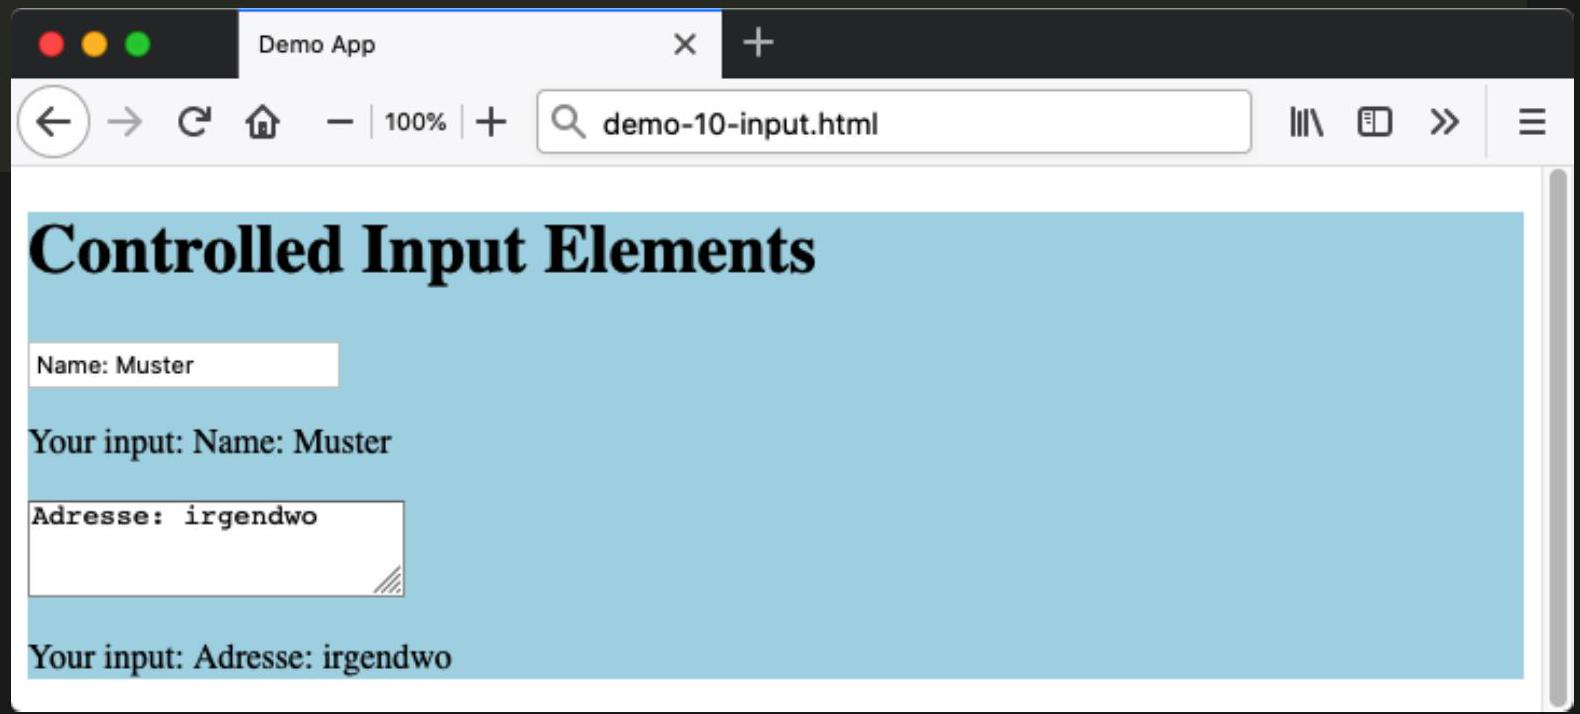
\includegraphics[max width=\textwidth]{2025_01_02_a730400f36f38fd94791g-17}
\end{center}

\section*{KONTROLLIERTE EINGABE}
\begin{itemize}
  \item Ermöglicht es, nur bestimmte Eingaben zu erlauben
  \item Beispiel: nur Ziffern und Dezimalpunkt erlaubt
\end{itemize}

\begin{verbatim}
const updateValue = e => {
    const inp = e.target.value
    const reg = /^\d+\.?\d*$/
    if (reg.test(inp)) setText(inp)
    else setText(text)
}
\end{verbatim}

\section*{ÜBERSICHT}
\begin{itemize}
  \item Zustand von Komponenten
  \item Komponenten-Design
  \item Optimierungsansätze
\end{itemize}

\section*{CONTAINER-KOMPONENTE}
\begin{itemize}
  \item Daten-Verwaltung von Daten-Darstellung trennen
  \item Container-Komponente zuständig, Daten zu holen
  \item Daten per props an Render-Komponenten weitergegeben
  \item Übliches Muster in React-Applikationen
\end{itemize}

\section*{BEISPIEL}
\begin{verbatim}
/* Utility function that's intended to mock a service that this
/* component uses to fetch it's data. It returns a promise, just
/* like a real async API call would. In this case, the data is
/* resolved after a 2 second delay. */
function fetchData() {
    return new Promise((resolve) => {
            setTimeout(() => {
            resolve([ 'First', 'Second', 'Third' ])
        }, 2000)
        })
}
\end{verbatim}

5

\section*{CONTAINER-KOMPONENTE}
\begin{verbatim}
const MyContainer = () => {
    let initialState = { items: ["Fetching data..."] }
    let [state, setState] = useState(initialState)
    if (state === initialState) {
        fetchData()
            .then(items => setState(() => ({ items })))
    }
    return (
        [MyList, state]
    )
}
\end{verbatim}

demo-25-container

\section*{EFFECT HOOK}
\begin{itemize}
  \item Container-Komponenten haben verschiedene Aufgaben
  \item Zum Beispiel: Timer starten, Daten übers Netz laden
  \item In React unterstützen Klassen-Komponenten zu diesem Zweck verschiedene Lifecycle-Methoden, u.a.:\\
componentDidMount: Komponente wurde gerendert componentWillUnmount: Komponente wird gleich entfernt
  \item In Funktionskomponenten: Effect Hooks
  \item Funktionen, die nach dem Rendern ausgeführt werden\\
\href{https://react.dev/learn/synchronizing-with-effects}{https://react.dev/learn/synchronizing-with-effects}
\end{itemize}

\section*{EFFECT HOOK}
\begin{verbatim}
const MyContainer = () => {
    // after the component has been rendered, fetch data
    useEffect(() => {
        fetchData()
            .then(items => setState(() => ({ items })))
    }, []) ...
}
\end{verbatim}

\begin{itemize}
  \item React.js-Beispiel
  \item Hier ist ein weiteres Beispiel:\\
\href{https://suiweb.github.io/docs/tutorial/4-hooks#indexjs}{https://suiweb.github.io/docs/tutorial/4-hooks\#indexjs}
\end{itemize}

\section*{MONOLITHISCHE KOMPONENTEN}
\begin{itemize}
  \item Design-Entscheidung: wie viel UI-Logik in einer Komponente?
  \item Einfaches UI in einer einzelnen Komponente realisieren?
  \item Damit: weniger Komponenten zu entwickeln und pflegen
  \item Und: weniger Kommunikation zwischen Komponenten
\end{itemize}

\section*{Aber:}
\begin{itemize}
  \item Wenig änderungsfreundlich
  \item Kaum Wiederverwendung von Komponenten
\end{itemize}

\section*{BEISPIEL-ANWENDUNG}


\begin{itemize}
  \item Artikel können hinzugefügt werden
  \item Artikel: Titel, Zusammenfassung
  \item Klick auf den Titel: Inhalt einund ausblenden
  \item Klick auf X: Artikel löschen
\end{itemize}

\section*{AUFTEILUNG IN KOMPONENTEN}
\section*{Articles}
\begin{itemize}
  \item Article $1 \underline{x}$
\end{itemize}

Article 1 Summary

\begin{itemize}
  \item Article $2 \underline{X}$
  \item Article 3 X
  \item Article 4 X
\end{itemize}

\section*{ArticleList}
\section*{Articleltem}
\section*{AUFTEILUNG IN KOMPONENTEN}
\begin{verbatim}
const App = () => {
let initialState = { ...}
let [state, setState] = useState(...)
const onChangeTitle = e => { ... }
const onChangeSummary = e => { ... }
const onClickAdd = e => { ... }
const onClickRemove = (id) => { ... }
const onClickToggle = (id) => { ... }
\end{verbatim}

\begin{verbatim}
    return
    ["section",
        [AddArticle, {
            name: "Articles",
            title: state.title,
            summary: state.summary,
            onChangeTitle,
            onChangeSummary,
            onClickAdd,
        }],
    [ArticleList, {
        articles: state.articles,
        onClickToggle,
        onClickRemove,
    }] ]
)
}
\end{verbatim}

\section*{AUFTEILUNG IN KOMPONENTEN}
\begin{itemize}
  \item Komponente App kümmert sich um den Zustand
  \item Sie enthält: Event Handler zum Anpassen des Zustands
  \item Ausgabe übernehmen AddArticle und ArticleList
  \item Diese bekommen dazu den Zustand und die Handler in Form von Properties übergeben
\end{itemize}

\section*{APPLIKATIONSZUSTAND}
\begin{verbatim}
const App = () => {
    let initialState = {
        articles: [
            {
                id: cuid(),
                title: 'Article 1',
                summary: 'Article 1 Summary',
                display: 'none',
            },
            •••
        ],
        title: '',
        summary: '',
    }
}
\end{verbatim}

\section*{],}
\begin{verbatim}
title:
summary: ',
\end{verbatim}

\begin{itemize}
  \item Array von Artikeln
  \item Generierte IDs
  \item title und summary für Eingabefelder (controlled input)
\end{itemize}

\section*{EREIGNISBEHANDLUNG}
\begin{verbatim}
const App = () => {
    let initialState = { ...}
    let [state, setState] = useState(initialState)
    const onChangeTitle = e => {
        setState({...state, title: e.target.value})
    }
    const onClickRemove = (id) => {
        let articles = state.articles.filter(a => a.id != id)
        setState({...state, articles})
    }
    /*...*/
    return (...)
}
\end{verbatim}

\section*{AUFTEILUNG IN KOMPONENTEN}
\begin{verbatim}
const AddArticle = ({name, title, summary,
    onChangeTitle, onChangeSummary, onClickAdd}) => (
    ["section",
        ["h1", name],
        ["input", { placeholder: "Title", value: title,
                oninput: onChangeTitle }],
    ["input", { placeholder: "Summary", value: summary,
            oninput: onChangeSummary }],
    ["button", { onclick: onClickAdd }, "Add"] ]
)
\end{verbatim}

\section*{AUFTEILUNG IN KOMPONENTEN}
\begin{verbatim}
const ArticleList = ({articles, onClickToggle, onClickRemove}) => (
    ["ul", ...articles.map(i => (
        [ArticleItem, {
            key: i.id,
            article: i,
            onClickToggle,
            onClickRemove} ]))]
)
\end{verbatim}

demo-26-design

\section*{AUFTEILUNG IN KOMPONENTEN}
\begin{itemize}
  \item Zustand in wenigen Komponenten konzentriert
  \item Andere Komponenten für den Aufbau des UI zuständig
  \item Im Beispiel: Zustandsobjekt enthält kompletten Applikationszustand (inkl. Inhalt der Eingabefelder)
  \item Event Handler passen diesen Zustand an und basteln nicht am DOM herum
\end{itemize}

\section*{MODULE}
\begin{itemize}
  \item Komponenten können in eigene Module ausgelagert werden
  \item Zusammen mit komponentenspezifischen Styles
  \item Sowie mit lokalen Hilfsfunktionen
\end{itemize}

\section*{Separation of Concerns}
\begin{itemize}
  \item Wo sollte getrennt werden?
  \item Zwischen Markup und Styles und Programmlogik?
  \item Zwischen Komponenten?
\end{itemize}

\section*{MODULE}
\begin{verbatim}
import { ArticleItem } from "./ArticleItem.js"
const ArticleList = ({articles, onClickToggle, onClickRemove}) => (
    ["ul", ...articles.map(i => (
        [ArticleItem, {
            key: i.id,
            article: i,
            onClickToggle,
            onClickRemove} ]))]
)
export { ArticleList }
\end{verbatim}

demo-27-modules

\section*{NETZWERKZUGRIFF}
\begin{itemize}
  \item Letztes Beispiel erweitert
  \item Falls Artikelliste leer: Button zum Laden vom Netz
  \item Dazu stellt unser Express-REST-Service unter der id articles eine Artikelliste mit ein paar Mustereinträgen zur Verfügung
\end{itemize}

\section*{NETZWERKZUGRIFF}
\begin{verbatim}
const App = () => {
    let [state, setState] = useState(initialState)
    /* ... */
    return (
        ["section",
            [AddArticle, { ... } ],
            state.articles.length != 0
            ? [ArticleList, {articles: state.articles, onClickToggle, onClickRemove}]
            : ["p", ["button", {onclick: onLoadData}, "Load Articles"]]
        ]
    )
}
\end{verbatim}

\section*{NETZWERKZUGRIFF}
\begin{verbatim}
// Load articles from server
const onLoadData = () => {
    let url = 'http://localhost:3000/'
    fetch(url + "api/data/articles?api-key=wbeweb", {
        method: 'GET',
    })
        .then(response => response.json())
    .then(articles => setState({...state, articles}))
    .catch(() => {alert("Network connection failed")})
}
\end{verbatim}

demo-28-network

\section*{IMPERATIVER ANSATZ}
Ergänze alle Code-Teile in denen die Artikelliste erweitert oder verkleinert wird wie folgt:

\begin{itemize}
  \item Wenn der letzte Artikel gelöscht wird, entferne <uıl></ul> und füge einen Button für den Netzwerkzugriff ein
  \item Wenn der erste Artikel eingefügt wird, entferne den Button und füge ein  mit dem ersten / ein
  \item usw.
\end{itemize}

\section*{DEKLARATIVER ANSATZ}
\begin{itemize}
  \item Wenn die Artikelliste leer ist, wird ein Button ausgegeben
  \item Ansonsten wird die Artikelliste ausgegeben
\end{itemize}

Wir ändern nur den Zustand...

\section*{HAUPTKONZEPTE}
\begin{itemize}
  \item Klarer und einfacher Datenfluss:
  \item Daten nach unten weitergegeben (props)
  \item Ereignisse nach oben weitergegeben und dort behandelt
  \item Properties werden nicht geändert, Zustand ist veränderbar
  \item Zustand wird von Komponente verwaltet
  \item Es ist von Vorteil, die meisten Komponenten zustandslos zu konzipieren
\end{itemize}

\section*{ÜBERSICHT}
\begin{itemize}
  \item Zustand von Komponenten
  \item Komponenten-Design
  \item Optimierungsansätze
\end{itemize}

\section*{OPTIMIERUNGSANSÄTZE}
\begin{itemize}
  \item SuiWeb ist nicht für den produktiven Einsatz gedacht
  \item Im Folgenden werden Optimierungsansätze beschrieben
  \item Diese sind in SuiWeb nur teilweise implementiert
  \item Angelehnt an:
\end{itemize}

\begin{verbatim}
Rodrigo Pombo: Build your own React
https://pomb.us/build-your-own-react/
Zachary Lee: Build Your Own React.js in 400 Lines of Code
https://webdeveloper.beehiiv.com/p/build-react-400-lines-code
\end{verbatim}

Die Optimierungen werden hier nur grob skizziert und gehören nicht zum WBE-Pflichtstoff. Bei Interesse bitte angegebene Quellen konsultieren.

\section*{OPTIMIERUNG}
\section*{Problem:}
Die render-Funktion blockiert den Browser, was besonders beim Rendern grösserer Baumstrukturen problematisch ist

\section*{Abhilfe:}
\begin{itemize}
  \item Zerlegen der Aufgabe in Teilaufgaben
  \item Aufruf mittels requestIdleCallback
  \item Achtung: experimentelle Technologie
  \item React selbst verwendet dafür mittlerweile ein eigenes Paket „FWIW we've since stopped using requestIdleCallback..." \href{https://github.com/facebook/react/issues/11171}{https://github.com/facebook/react/issues/11171}
\end{itemize}

\section*{OPTIMIERUNG}
\begin{verbatim}
let nextUnitOfWork = null
function workLoop (deadline) {
    let shouldYield = false
    while (nextUnitOfWork && !shouldYield) {
        nextUnitOfWork = performUnitOfWork(
            nextUnitOfWork
        )
        shouldYield = deadline.timeRemaining() < 1
    }
    requestIdleCallback(workLoop)
}
requestIdleCallback(workLoop)
function performUnitOfWork (nextUnitOfWork) {
    // TODO
}
\end{verbatim}

\section*{OPTIMIERUNG: FIBERS}
\begin{itemize}
  \item Offen: wie wird das Rendern in Teilaufgaben zerlegt?
  \item Datenstruktur: Fiber Tree
  \item Ziel: einfaches Auffinden des nächsten Arbeitsschritts
  \item Fiber heisst eigentlich Faser
  \item Terminologie hier: Arbeitspaket (eigentlich: Unter-/Teilauftrag)
\end{itemize}

\section*{FIBERS: DATENSTRUKTUR}
[div, [h1, p, a], h2]

\begin{itemize}
  \item Elemente geeignet verlinkt
  \item Jedes Arbeitspaket kennt
  \item erstes Kind (first child)
  \item nächstes Geschwister (next sibling)
  \item übergeordnetes Element (parent)
\end{itemize}

\section*{FIBERS: NÄCHSTER SCHRITT}
\begin{itemize}
  \item Kind falls vorhanden
  \item sonst: nächstes Geschwister falls vorhanden
  \item sonst: Suche nach oben bis Element mit Geschwister
  \item sonst: fertig
\end{itemize}

\section*{FIBERS: IMPLEMENTIERUNG}
\begin{itemize}
  \item Funktion render aufgeteilt
  \item Legt nun erstes Arbeitspaket fest
  \item In createDom wird DOM-Knoten mit Attributen angelegt
\end{itemize}

\begin{verbatim}
let nextUnitOfWork = nul1
function render (element, container) {
    // erstes Arbeitspaket festlegen
}
function workLoop (deadline) {
    // Arbeitspakete bearbeiten
}
\end{verbatim}

\section*{FIBERS: IMPLEMENTIERUNG}
\begin{itemize}
  \item Noch offen: performUnitOfWork
  \item Bearbeitet aktuellen Auftrag und liefert nächsten Auftrag
  \item Dieser wird im while gleich bearbeitet, falls Browser idle
  \item Sonst im nächsten requestIdleCall.back
\end{itemize}

\begin{verbatim}
function performUnitOfWork (fiber) {
    // TODO add dom node
    // TODO create new fibers
    // TODO return next unit of work
}
\end{verbatim}

\section*{FIBERS: IMPLEMENTIERUNG}
\begin{verbatim}
function performUnitOfWork(fiber) {
    // TODO add dom node
    // TODO create new fibers
    // TODO return next unit of work
}
\end{verbatim}

\begin{itemize}
  \item Knoten anlegen ( createDom) und ins DOM einhängen
  \item Für jedes Kindelement Arbeitspaket (Fiber) anlegen
  \item Referenzen eintragen (sibling, parent, child)
  \item Nächstes Arbeitspaket suchen und zurückgeben
\end{itemize}

\section*{AUFTEILUNG IN ZWEI PHASEN}
\section*{Erste Phase:}
\begin{itemize}
  \item Fibers anlegen
  \item DOM-Knoten anlegen (dom-Attribut)
  \item Properties hinzufügen
  \item Fibers verlinken: parent, child, sibling
\end{itemize}

\section*{Zweite Phase:}
\begin{itemize}
  \item DOM-Teil der Fibers (. .dom ) ins DOM hängen
\end{itemize}

Implementierung: s. Step V: Render and Commit Phases\\
\href{https://pomb.us/build-your-own-react/}{https://pomb.us/build-your-own-react/}

\section*{ABGLEICH MIT LETZTER VERSION}
\begin{itemize}
  \item Ziel: nur Änderungen im DOM nachführen
  \item Referenz auf letzte Version des Fiber Tree: currentRoot
  \item Jedes Fiber erhält Referenz auf letzte Version: alternate
  \item Nach der Aktualisierung wird aktuelle zur letzten Version
  \item Unterscheidung von update - und placement -Fibers
  \item Ausserdem eine Liste der zu löschenden Knoten
\end{itemize}

Didact: (Rodrigo Pombo)\\
\href{https://codesandbox.io/s/didact-6-96533}{https://codesandbox.io/s/didact-6-96533}

\section*{QUELLENANGABEN}
\begin{itemize}
  \item Beispiele angeleht an:
\end{itemize}

Adam Boduch: React and React Native Second Edition, Packt Publishing, 2018 Packt Online Shop

\begin{itemize}
  \item Rodrigo Pombo: Build your own React \href{https://pomb.us/build-your-own-react/}{https://pomb.us/build-your-own-react/}
  \item Zachary Lee: Build Your Own React.js in 400 Lines of Code \href{https://webdeveloper.beehiiv.com/p/build-react-400-lines-code}{https://webdeveloper.beehiiv.com/p/build-react-400-lines-code}
\end{itemize}

\section*{WEITERE INFORMATIONEN}
\begin{itemize}
  \item Rodrigo Pombo: Build your own React \href{https://pomb.us/build-your-own-react/}{https://pomb.us/build-your-own-react/}
  \item Zachary Lee: Build Your Own React.js in 400 Lines of Code \href{https://webdeveloper.beehiiv.com/p/build-react-400-lines-code}{https://webdeveloper.beehiiv.com/p/build-react-400-lines-code}
  \item SuiWeb - An Educational Web Framework (Inspired by React) \href{https://github.com/suiweb/suiweb}{https://github.com/suiweb/suiweb}
\end{itemize}

\section*{Stand:}
7.12.2024 12:24


\end{document}